\documentclass[11pt]{article}

\usepackage[T1]{fontenc}
\usepackage{lmodern}
\usepackage{microtype}
\usepackage[margin=0.92in,headheight=14pt]{geometry}
\usepackage{amsmath,amssymb,amsthm,mathtools}
\usepackage{bm}
\usepackage{xcolor}
\usepackage{enumitem}
\usepackage{booktabs,tabularx,array}
\usepackage{tikz}
\usetikzlibrary{arrows.meta,positioning,calc,decorations.pathreplacing}
\usepackage[most]{tcolorbox}
\usepackage{fancyhdr}
\usepackage{hyperref}
\usepackage[nameinlink,noabbrev]{cleveref}

\definecolor{navy}{HTML}{17365D}
\definecolor{teal}{HTML}{117A8B}
\definecolor{ink}{HTML}{2C3138}
\definecolor{lightblue}{HTML}{EEF5FA}
\definecolor{lightgray}{HTML}{F4F5F7}
\definecolor{softgreen}{HTML}{EEF7F2}
\definecolor{greenframe}{HTML}{3C735B}
\definecolor{warm}{HTML}{FFF7E8}
\definecolor{warmframe}{HTML}{A86E20}

\hypersetup{
  colorlinks=true,
  linkcolor=navy,
  citecolor=teal,
  urlcolor=teal,
  pdftitle={Continuum Petz Recovery for Adjacent Intervals in the Free Chiral Fermion},
  pdfauthor={Technical research note}
}

\pagestyle{fancy}
\fancyhf{}
\fancyhead[L]{\small\color{ink}Continuum Petz recovery}
\fancyhead[R]{\small\color{ink}Free chiral fermion}
\fancyfoot[C]{\small\thepage}
\renewcommand{\headrulewidth}{0.4pt}

\newtheoremstyle{accent}
  {8pt}{8pt}{\itshape}{}
  {\color{navy}\bfseries}{.}{0.5em}{}
\theoremstyle{accent}
\newtheorem{theorem}{Theorem}[section]
\newtheorem{proposition}[theorem]{Proposition}
\newtheorem{lemma}[theorem]{Lemma}
\newtheorem{corollary}[theorem]{Corollary}

\theoremstyle{definition}
\newtheorem{definition}[theorem]{Definition}
\newtheorem{remark}[theorem]{Remark}

\newcommand{\cF}{\mathcal{F}}
\newcommand{\cA}{\mathcal{A}}
\newcommand{\cB}{\mathcal{B}}
\newcommand{\cM}{\mathfrak{M}}
\newcommand{\cN}{\mathfrak{N}}
\newcommand{\cR}{\mathcal{R}}
\newcommand{\CAR}{\operatorname{CAR}}
\newcommand{\id}{\operatorname{id}}
\newcommand{\Ad}{\operatorname{Ad}}
\newcommand{\Tr}{\operatorname{Tr}}
\newcommand{\Ran}{\operatorname{Ran}}
\newcommand{\supp}{\operatorname{supp}}
\newcommand{\pv}{\operatorname{pv}}
\newcommand{\dd}{\,\mathrm{d}}
\newcommand{\eps}{\varepsilon}
\newcommand{\one}{\mathbf{1}}
\newcommand{\Sone}{\mathfrak{S}_1}
\newcommand{\Stwo}{\mathfrak{S}_2}
\newcommand{\Fid}{\operatorname{F}}
\newcommand{\MI}{\operatorname{MI}}
\newcommand{\CMI}{I}
\newcommand{\norm}[1]{\left\lVert #1\right\rVert}
\newcommand{\abs}[1]{\left|#1\right|}
\newcommand{\ip}[2]{\left\langle #1,#2\right\rangle}

\newtcolorbox{mainbox}{
  enhanced,
  colback=lightblue,
  colframe=navy,
  boxrule=0.85pt,
  arc=2mm,
  left=5mm,right=5mm,top=3.8mm,bottom=3.8mm,
  title={\bfseries Main result},
  coltitle=white,
  colbacktitle=navy,
  attach boxed title to top left={xshift=4mm,yshift=-2mm}
}

\newtcolorbox{proofbox}[1][]{
  enhanced,
  breakable,
  colback=softgreen,
  colframe=greenframe,
  boxrule=0.65pt,
  arc=1.5mm,
  left=4mm,right=4mm,top=2.8mm,bottom=2.8mm,
  title={\bfseries #1},
  coltitle=white,
  colbacktitle=greenframe
}

\newtcolorbox{caveatbox}{
  enhanced,
  breakable,
  colback=warm,
  colframe=warmframe,
  boxrule=0.65pt,
  arc=1.5mm,
  left=4mm,right=4mm,top=2.8mm,bottom=2.8mm,
  title={\bfseries Precise scope},
  coltitle=white,
  colbacktitle=warmframe
}

\setlist[itemize]{leftmargin=1.5em,itemsep=2.5pt,topsep=4pt}
\setlist[enumerate]{leftmargin=1.8em,itemsep=3pt,topsep=4pt}
\setlength{\parindent}{0pt}
\setlength{\parskip}{5.2pt}
\allowdisplaybreaks
\emergencystretch=2em
\raggedbottom

\title{\vspace{-1.55cm}\color{navy}\bfseries
Continuum Petz Recovery for Adjacent Intervals\\[0.25em]
\Large in the Free Chiral Fermion\\[0.5em]
\large Half-sided modular geometry, an exact trace-class endpoint estimate,\\
and zero-collar normality}
\author{}
\date{}

\begin{document}
\maketitle
\vspace{-1.55em}

\begin{abstract}
Let \(A=(-a,0)\), \(B=(0,b)\), and \(C=(b,b+c)\) be adjacent intervals, and let \(\omega\) be the vacuum of the \(r\)-component chiral free-fermion net.  A positive collar between \(A\) and \(B\) makes the usual split-product reference state available, so the Faulkner--Hollands--Swingle--Wang rotated Petz map is well defined.  The nontrivial factor is the vacuum inclusion \(\cF_r(B)\subset\cF_r(BC)\), which is a half-sided modular inclusion.  Its rotated Petz maps are geometric compressions of \(BC\) into subintervals of \(B\).  The collar maps therefore glue at the CAR \(C^*\)-algebra level to a piecewise geometric map on \(ABC\).  The central calculation of this note proves that the difference between the true and recovered one-particle covariances is trace class.  After inversion at the touching endpoint, its off-diagonal block becomes a positive difference of two shifted Carleman--Hankel operators.  A rank-one Laplace factorization gives the exact trace norm.  The Powers--St\o rmer--Araki criterion then implies quasi-equivalence, hence the glued map extends normally to the touching type-III local algebra.  Finally, the Longo--Xu conditional mutual information controls the fidelity of the normal twirled zero-collar channel.
\end{abstract}

\begin{center}
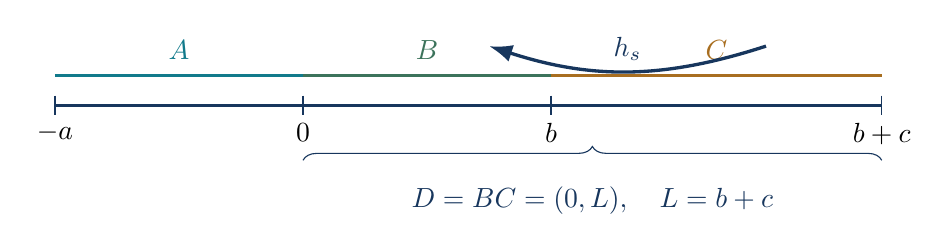
\begin{tikzpicture}[x=1.05cm,y=1cm,>=Latex]
  \draw[very thick,navy] (0,0)--(10,0);
  \foreach \x/\lab in {0/{-a},3/0,6/b,10/{b+c}}{
    \draw[navy] (\x,0.12)--(\x,-0.12);
    \node[below=3pt] at (\x,0) {$\lab$};
  }
  \draw[very thick,teal] (0,0.38)--(3,0.38);
  \draw[very thick,greenframe] (3,0.38)--(6,0.38);
  \draw[very thick,warmframe] (6,0.38)--(10,0.38);
  \node[above=2pt,teal] at (1.5,0.38) {$A$};
  \node[above=2pt,greenframe] at (4.5,0.38) {$B$};
  \node[above=2pt,warmframe] at (8,0.38) {$C$};
  \draw[decorate,decoration={brace,amplitude=5pt},navy] (3,-0.7)--(10,-0.7)
    node[midway,below=6pt] {$D=BC=(0,L),\quad L=b+c$};
  \draw[->,very thick,navy,bend left=18] (8.6,0.75) to node[above] {$h_s$} (5.25,0.75);
\end{tikzpicture}
\end{center}

\begin{mainbox}
Put
\[
 L=b+c,\qquad z=\frac{ac}{b(a+b+c)},\qquad
 \eta=\frac{b(a+b+c)}{(a+b)(b+c)}=\frac1{1+z}.
\]
For the ordinary Petz map, the zero-collar recovered quasi-free covariance \(\widetilde Q_{\mathrm P}\) satisfies
\[
 Q_{ABC}-\widetilde Q_{\mathrm P}\in\Sone,
 \qquad
 \boxed{
 \norm{Q_{ABC}-\widetilde Q_{\mathrm P}}_1
 =\frac{r}{2\pi}\log(1+2z).
 }
\]
Equivalently, for the cross-correlation block,
\[
 \boxed{
 \norm{Q_{A,BC}-\widetilde Q_{A,BC}}_1
 =\frac{r}{4\pi}\log(1+2z).
 }
\]
Hence the recovered state is normal in the vacuum representation and the collar Petz maps are restrictions of a normal \(*\)-homomorphism
\[
 \overline\beta_{\mathrm P}:\cF_r(ABC)\longrightarrow\cF_r(AB).
\]
Longo--Xu give
\[
 \CMI_\omega(A:C\mid B)=\frac r6\log(1+z)=-\frac r6\log\eta.
\]
Thus the covariance trace norm obeys the exact identity
\[
 \norm{Q_{ABC}-\widetilde Q_{\mathrm P}}_1
 =\frac{r}{2\pi}
 \log\!\left(2e^{6\CMI_\omega(A:C\mid B)/r}-1\right).
\]
The left side is a one-particle Schatten norm; it is \emph{not} the predual norm distance between the two states.
\end{mainbox}

\begin{caveatbox}
At zero collar there is no normal product state \(\omega_A\otimes\omega_{BC}\) on the touching local algebra.  Accordingly, \(\overline\beta_t\) is not described as the Petz map of a nonexistent zero-collar product reference state.  It is the unique normal extension of the compatible positive-collar Petz maps.  All statements below are for the graded free-fermion field net; because the maps preserve parity, they restrict to the even observable subnet.
\end{caveatbox}

\tableofcontents
\clearpage

\section{Setup and external inputs}

\subsection{The vacuum covariance}

Let
\[
 I=ABC=(-a,L),\qquad A=(-a,0),\qquad D=BC=(0,L),
\]
with \(a,b,c>0\) and \(L=b+c\).  The one-particle space is
\[
 H=L^2(\mathbb R;\mathbb C^r).
\]
Let \(P_+\) be the Hardy projection.  With the Fourier convention \(\hat f(k)=\int f(x)e^{-ikx}\,dx\), under which \(P_+\) is the projection onto \(\{k<0\}\), the positive-energy subspace for the light-ray coordinate used here, its distributional kernel is
\begin{equation}\label{eq:hardy-kernel}
 P_+(x,y)
 =\frac12\delta(x-y)-\frac{i}{2\pi}\pv\frac1{x-y}.
\end{equation}
For a bounded interval \(X\), write \(E_X\) for multiplication by \(\mathbf 1_X\) and set
\begin{equation}\label{eq:local-symbol}
 Q_X=E_XP_+E_X\big|_{L^2(X;\mathbb C^r)}.
\end{equation}
The vacuum restricted to \(\CAR(L^2(X;\mathbb C^r))\) is the gauge-invariant quasi-free state with symbol \(Q_X\):
\begin{equation}\label{eq:qf-two-point}
 \omega\bigl(a^*(f)a(g)\bigr)=\ip{g}{Q_Xf}.
\end{equation}
Longo and Xu's net \(\mathcal A_r=\mathrm{CAR}(L^2(\mathbb R,\mathbb C^r))\) consists of \(r\) complex chiral fermions with central charge \(c=r\), and they use this Hardy-projection realization to compute the Araki relative entropy and mutual information of separated free-fermion intervals \cite{LongoXu}.

\subsection{Modular geometry and recovery}

We use the following established results.

\begin{enumerate}
  \item The vacuum modular group of an interval algebra in a conformal net is the one-parameter M\"obius group preserving that interval; see Brunetti--Guido--Longo \cite{BGL}.
  \item An inclusion of interval algebras with one common endpoint is half-sided modular; for a common left endpoint, as for \(\cF_r(B)\subset\cF_r(D)\) below, it is a \(+\)hsm inclusion in Wiesbrock's convention, i.e.\ the Borchers translations \(U(s)\), \(s\ge0\), map \(\cF_r(D)\) into itself and satisfy \(\Delta^{it}U(s)\Delta^{-it}=U(e^{2\pi t}s)\), \(JU(s)J=U(-s)\).  The associated Borchers translation is described by Wiesbrock's theory \cite{Wiesbrock}.
  \item For a half-sided modular inclusion, Faulkner--Hollands--Swingle--Wang identify every rotated Petz map with a member of the Borchers translation semigroup \cite[Sec.~4.2]{FHWS}.
  \item Gauge-invariant quasi-free CAR representations with symbols \(S,T\) are quasi-equivalent exactly when
  \[
    S^{1/2}-T^{1/2}\in\Stwo,
    \qquad
    (1-S)^{1/2}-(1-T)^{1/2}\in\Stwo;
  \]
  see Powers--St\o rmer and Araki \cite{PowersStormer,ArakiCAR}.
\end{enumerate}

The first three inputs determine the recovery map.  The fourth converts the endpoint trace-class calculation into normality on the type-III local algebra.

\section{The half-sided modular Petz map for \texorpdfstring{\(B\subset BC\)}{B contained in BC}}

\subsection{The translation coordinate}

On \(D=(0,L)\), define
\begin{equation}\label{eq:q-coordinate}
 q(x)=\frac{L-x}{x}.
\end{equation}
It is a decreasing bijection from \(D\) onto \((0,\infty)\).  Since
\[
 q(b)=\frac{L-b}{b}=\frac cb,
\]
put
\begin{equation}\label{eq:lambda}
 \lambda=\frac cb.
\end{equation}
Then
\[
 q(B)=(\lambda,\infty).
\]
Translation by \(s\ge0\) in the \(q\)-coordinate induces the fractional-linear map
\begin{equation}\label{eq:h-s}
 q(h_s(x))=q(x)+s,
 \qquad
 \boxed{h_s(x)=\frac{Lx}{L+sx}}.
\end{equation}
Its derivative and semigroup law are
\begin{equation}\label{eq:h-derivative-semigroup}
 h_s'(x)=\frac{L^2}{(L+sx)^2},
 \qquad
 h_s\circ h_t=h_{s+t}.
\end{equation}
Moreover,
\begin{equation}\label{eq:D-s}
 D_s:=h_s(D)=\left(0,\frac{L}{1+s}\right),
 \qquad
 D_\lambda=(0,b)=B.
\end{equation}
Let
\[
 \gamma_s:\cF_r(D)\longrightarrow\cF_r(D_s)
\]
be the vacuum-covariant M\"obius homomorphism induced by \(h_s\).  The inclusion \(\cF_r(B)=\gamma_\lambda(\cF_r(D))\subset\cF_r(D)\) is half-sided modular (\(+\)hsm, common left endpoint \(0\)).

\subsection{Ordinary and rotated Petz maps}

For clarity, first consider the ordinary Petz map.  In a standard half-sided modular inclusion
\[
 \cB=U(\lambda)\cA U(\lambda)^*\subset\cA,
\]
the common vacuum vector is cyclic and separating and the standard-form embedding is the identity.  Hence the Petz generalized conditional expectation is
\[
 \alpha_0(x)=J_{\cB}J_{\cA}xJ_{\cA}J_{\cB}.
\]
Vacuum covariance gives
\[
 J_{\cB}=U(\lambda)J_{\cA}U(\lambda)^*,
 \qquad
 J_{\cA}U(s)J_{\cA}=U(-s).
\]
Therefore
\[
 J_{\cB}=U(2\lambda)J_{\cA},
 \qquad
 \alpha_0(x)=U(2\lambda)xU(2\lambda)^*.
\]
In the geometric orientation fixed by \eqref{eq:h-s}, this is \(\gamma_{2\lambda}\).

Faulkner--Hollands--Swingle--Wang give the rotated family.  We use the modular-time convention
\begin{equation}\label{eq:s-t}
 \boxed{
 s_t=\lambda\bigl(1+e^{-2\pi t}\bigr),
 \qquad
 \alpha_t^{D\to B}=\gamma_{s_t}.
 }
\end{equation}
\noindent(For comparison with the source: FHSW's printed eq.~(167) is inconsistent with their own (25), (166) and (22): as printed it maps \(\mathcal A\) out of \(\mathcal B\), and ``for \(t\ge0\)'' must read \(t\le0\); documented with screenshot in \texttt{rigor/check\_note4.tex}, Thm~3.8.  Nothing here relies on the printed formula.)
Explicitly, with \(\alpha_t=\sigma^{\cN}_{-t}\circ\alpha_0\circ\sigma^{\cM}_t\), \(\sigma_t=\operatorname{Ad}\Delta^{it}\), the \(+\)hsm relation \(\Delta_{\cM}^{-it}U(s)\Delta_{\cM}^{it}=U(e^{-2\pi t}s)\) and \(\Delta_{\cN}=U(\lambda)\Delta_{\cM}U(\lambda)^*\), one has \(\Delta_{\cN}^{-it}U(2\lambda)\Delta_{\cM}^{it}=U(\lambda)\Delta_{\cM}^{-it}U(\lambda)\Delta_{\cM}^{it}=U(\lambda)U(e^{-2\pi t}\lambda)=U(s_t)\).  Writing \(\alpha_t=\sigma^{\cN}_{t}\circ\alpha_0\circ\sigma^{\cM}_{-t}\) instead replaces \(t\) by \(-t\); since the twirling density \(p(t)\) below is even, nothing depends on this choice.  Since \(s_t\ge\lambda\),
\[
 D_{s_t}\subset D_\lambda=B,
\]
so \(\alpha_t^{D\to B}\) indeed maps \(\cF_r(D)\) into \(\cF_r(B)\).  At \(t=0\),
\begin{equation}\label{eq:s-P}
 \boxed{s_{\mathrm P}=2\lambda=\frac{2c}{b}.}
\end{equation}

\subsection{One-particle formula}

Let \(H_D=L^2(D;\mathbb C^r)\).  Define the half-density push-forward
\begin{equation}\label{eq:V-def}
 (V_sf)(z)
 =\frac{f(h_s^{-1}(z))}
 {\sqrt{h_s'(h_s^{-1}(z))}},
 \qquad z\in D_s.
\end{equation}
Since
\[
 h_s^{-1}(z)=\frac{Lz}{L-sz},
\]
we have the explicit formula
\begin{equation}\label{eq:V-explicit}
 \boxed{
 (V_sf)(z)=\frac{L}{L-sz}
 f\!\left(\frac{Lz}{L-sz}\right),
 \qquad 0<z<\frac{L}{1+s}.
 }
\end{equation}

\begin{lemma}\label{lem:V-isometry}
The map \(V_s:H_D\to L^2(D_s;\mathbb C^r)\) is unitary (an isometry onto all of \(L^2(D_s;\mathbb C^r)\), as used below) and
\[
 V_s^*V_s=1_{H_D}.
\]
\end{lemma}

\begin{proof}
With \(z=h_s(x)\), one has \(\dd z=h_s'(x)\dd x\), and therefore
\[
 \int_{D_s}\abs{(V_sf)(z)}^2\dd z
 =\int_D\frac{\abs{f(x)}^2}{h_s'(x)}h_s'(x)\dd x
 =\int_D\abs{f(x)}^2\dd x.
\]
Surjectivity onto \(L^2(D_s)\) follows by applying the inverse half-density transformation.
\end{proof}

On CAR generators,
\begin{equation}\label{eq:alpha-fields}
 \boxed{
 \alpha_t^{D\to B}\bigl(a(f)\bigr)=a(V_{s_t}f).
 }
\end{equation}
Because the vacuum is M\"obius invariant,
\begin{equation}\label{eq:reference-recovery}
 \omega_B\circ\alpha_t^{D\to B}=\omega_D.
\end{equation}
In quasi-free channel terminology the noise is zero: the Heisenberg map is a \(*\)-homomorphism induced by an isometry.

\section{Positive-collar factorization}

For \(0<\eps<a\), let
\[
 A_\eps=(-a,-\eps),
\]
and define
\begin{equation}\label{eq:collar-algebras}
 \cM_\eps=\cF_r(A_\eps)\vee\cF_r(D),
 \qquad
 \cN_\eps=\cF_r(A_\eps)\vee\cF_r(B).
\end{equation}
The split property gives the graded tensor-product identifications
\begin{equation}\label{eq:split-identifications}
 \cM_\eps\simeq\cF_r(A_\eps)\,\overline\otimes_{\mathrm{gr}}\,\cF_r(D),
 \qquad
 \cN_\eps\simeq\cF_r(A_\eps)\,\overline\otimes_{\mathrm{gr}}\,\cF_r(B).
\end{equation}
For parity-preserving maps one may equivalently use the usual Klein transform and ordinary tensor products: Longo--Xu's Lemma~3.1 identifies \(\cM_\eps\) with an ordinary tensor product after conjugating the \(D\)-factor by the Klein unitary, \(\sigma_\eps\) is the unique normal state factorizing on \(\cF_r(A_\eps)\times\cF_r(D)\) (it is faithful), and the Petz maps computed below are parity preserving; all statements of this section are to be read with this identification (verification document \texttt{rigor/check\_note4.tex}).  Let
\begin{equation}\label{eq:sigma-eps}
 \sigma_\eps=\omega_{A_\eps}\otimes\omega_D.
\end{equation}
Its restriction to \(\cN_\eps\) is \(\omega_{A_\eps}\otimes\omega_B\).

\begin{lemma}[Tensorization of the Petz map]\label{lem:tensorization}
The rotated Petz map for \(\cN_\eps\subset\cM_\eps\) with reference state \(\sigma_\eps\) is
\begin{equation}\label{eq:collar-map}
 \boxed{
 \alpha_{\eps,t}
 =\id_{\cF_r(A_\eps)}\,\overline\otimes\,\alpha_t^{D\to B}.
 }
\end{equation}
In particular, the nontrivial factor is independent of \(\eps\).
\end{lemma}

\begin{proof}
For product standard forms,
\[
 J_{A_\eps D}=J_{A_\eps}\otimes J_D,
 \qquad
 \Delta_{\sigma_\eps}=\Delta_{\omega_{A_\eps}}\otimes\Delta_{\omega_D},
\]
and the standard-form isometry for the inclusion is \(1\otimes V_{B\subset D}\).  Substitution into the Petz formula
\[
 \alpha_0(x)=J_{\cN}V^*J_{\cM}xJ_{\cM}VJ_{\cN}
\]
gives \(\id\otimes\alpha_0^{D\to B}\) on elementary tensors.  The modular rotations also factor, giving \eqref{eq:collar-map}; normality extends the identity to the von Neumann tensor product.
\end{proof}

\section{The glued zero-collar CAR map}

For fixed \(s\ge\lambda\), define the piecewise map
\begin{equation}\label{eq:k-s}
 k_s(x)=
 \begin{cases}
 x,&-a<x\le0,\\[1mm]
 h_s(x)=\dfrac{Lx}{L+sx},&0\le x<L.
 \end{cases}
\end{equation}
It maps \(I=(-a,L)\) bijectively onto
\begin{equation}\label{eq:J-s}
 J_s=\left(-a,\frac{L}{1+s}\right)\subset(-a,b)=AB.
\end{equation}
Since \(h_s(0)=0\) and \(h_s'(0)=1\), the two branches join with one derivative; in fact \(k_s\in C^{1,1}(I)\).

Let
\[
 H_I=L^2(I;\mathbb C^r)=H_A\oplus H_D,
 \qquad
 H_{J_s}=H_A\oplus L^2(D_s;\mathbb C^r),
\]
and set
\begin{equation}\label{eq:W-s}
 W_s=1_{H_A}\oplus V_s.
\end{equation}
This is the half-density push-forward induced by \(k_s\), and it is unitary from \(H_I\) onto \(H_{J_s}\).  The CAR functor therefore gives a parity-preserving \(C^*\)-isomorphism
\begin{equation}\label{eq:beta-Cstar}
 \boxed{
 \beta_s:\CAR(H_I)\longrightarrow\CAR(H_{J_s}),
 \qquad
 \beta_s(a(f))=a(W_sf).
 }
\end{equation}
For every \(\eps>0\), its restriction to the collar algebra is precisely the map in \cref{lem:tensorization} with \(s=s_t\).

Define the pulled-back vacuum state
\begin{equation}\label{eq:omega-tilde}
 \widetilde\omega_s=\omega_{J_s}\circ\beta_s.
\end{equation}
It is quasi-free with symbol
\begin{equation}\label{eq:Q-tilde}
 \widetilde Q_s=W_s^*Q_{J_s}W_s
\end{equation}
on \(H_I\).  The remaining task is to prove that \(\widetilde\omega_s\) is normal in the vacuum representation of \(\CAR(H_I)\).

\section{Exact covariance defect}

Decompose \(H_I=H_A\oplus H_D\).  The diagonal blocks of \(Q_I\) and \(\widetilde Q_s\) agree.

On \(A\times A\), this is immediate because \(k_s\) is the identity.  On \(D\times D\), the fractional-linear identity
\begin{equation}\label{eq:mobius-cauchy}
 \frac{\sqrt{h_s'(x)h_s'(y)}}{h_s(x)-h_s(y)}=\frac1{x-y}
\end{equation}
shows that the Cauchy kernel is unchanged; the \(\delta\)-term is invariant as well, since \(\delta(h_s(x)-h_s(y))=\delta(x-y)/h_s'(x)\) is compensated by the half-density factors, and the principal-value prescription is preserved by the M\"obius substitution.  Indeed,
\[
 h_s(x)-h_s(y)=\frac{L^2(x-y)}{(L+sx)(L+sy)},
 \qquad
 \sqrt{h_s'(x)h_s'(y)}=\frac{L^2}{(L+sx)(L+sy)}.
\]
Thus
\begin{equation}\label{eq:block-form}
 Q_I-\widetilde Q_s
 =\begin{pmatrix}
 0&\Delta_s\\
 \Delta_s^*&0
 \end{pmatrix}.
\end{equation}

To compute \(\Delta_s\), write \(x=-u\in A\) and \(y=v\in D\), where
\[
 0<u<a,\qquad0<v<L.
\]
By \eqref{eq:hardy-kernel}, the true vacuum cross-kernel is
\begin{equation}\label{eq:true-cross}
 Q_I(-u,v)=\frac{i}{2\pi}\frac1{u+v}.
\end{equation}
The recovered cross-kernel is
\begin{align}
 \widetilde Q_s(-u,v)
 &=-\frac{i}{2\pi}
 \frac{\sqrt{h_s'(v)}}{-u-h_s(v)}\notag\\
 &=\frac{i}{2\pi}
 \frac{L}{L(u+v)+suv}.
 \label{eq:recovered-cross}
\end{align}
Hence
\begin{equation}\label{eq:delta-kernel}
 \boxed{
 \Delta_s(-u,v)=\frac{i}{2\pi}R_s(u,v),
 \qquad
 R_s(u,v)=
 \frac{suv}{(u+v)\bigl(L(u+v)+suv\bigr)}.
 }
\end{equation}
Equivalently,
\begin{equation}\label{eq:R-difference}
 R_s(u,v)=\frac1{u+v}
 -\frac{L}{L(u+v)+suv}.
\end{equation}
The separate terms have the endpoint singularity \((u+v)^{-1}\); their difference is bounded.  Trace class requires a stronger argument.

\section{Hankel reduction and exact trace norm}

Regard \(R_s\) as the integral operator
\[
 R_s:L^2(0,L)\longrightarrow L^2(0,a)
\]
with kernel \eqref{eq:delta-kernel} without the factor \(i/(2\pi)\).

\subsection{Inversion at the touching endpoint}

For \(d>0\), define
\begin{equation}\label{eq:J-d}
 \mathcal J_d:L^2(0,d)\longrightarrow L^2(d^{-1},\infty),
 \qquad
 (\mathcal J_df)(p)=\frac1p f\!\left(\frac1p\right).
\end{equation}

\begin{lemma}\label{lem:J-unitary}
The map \(\mathcal J_d\) is unitary.
\end{lemma}

\begin{proof}
The substitution \(u=p^{-1}\) gives
\[
 \int_{1/d}^{\infty}\frac1{p^2}
 \abs{f(p^{-1})}^2\dd p
 =\int_0^d\abs{f(u)}^2\dd u.
\]
The inverse is given by the same formula with the variables interchanged.
\end{proof}

The integral kernel of \(\mathcal J_aR_s\mathcal J_L^*\) is
\begin{equation}\label{eq:inverted-kernel-start}
 \frac{R_s(p^{-1},q^{-1})}{pq}.
\end{equation}
A direct substitution into \eqref{eq:delta-kernel} gives
\begin{equation}\label{eq:inverted-kernel}
 \boxed{
 \frac{R_s(p^{-1},q^{-1})}{pq}
 =\frac{s}{(p+q)\bigl(L(p+q)+s\bigr)}.
 }
\end{equation}
Translate
\[
 p=\frac1a+x,\qquad q=\frac1L+y,
 \qquad x,y>0,
\]
and define
\begin{equation}\label{eq:alpha-beta}
 \alpha=\frac{s}{L},
 \qquad
 \beta=\frac1a+\frac1L.
\end{equation}
The operator becomes the Hankel operator on \(L^2(0,\infty)\) with kernel
\begin{equation}\label{eq:H-kernel}
 \boxed{
 H_{\alpha,\beta}(x,y)
 =\frac1{x+y+\beta}
 -\frac1{x+y+\beta+\alpha}.
 }
\end{equation}
Thus \(R_s\) and \(H_{\alpha,\beta}\) have the same singular values.

\subsection{Trace-norm convergent rank-one factorization}

For \(\rho>0\), set
\[
 e_\rho(x)=e^{-\rho x},\qquad x>0.
\]
Then
\begin{equation}\label{eq:e-rho-norm}
 \norm{e_\rho}_2^2=\frac1{2\rho}.
\end{equation}
The elementary Laplace formula gives
\begin{align}
 H_{\alpha,\beta}(x,y)
 &=\int_0^\infty
 e^{-\rho(x+y+\beta)}
 \bigl(1-e^{-\alpha\rho}\bigr)\dd\rho\notag\\
 &=\int_0^\infty
 e^{-\beta\rho}\bigl(1-e^{-\alpha\rho}\bigr)
 e_\rho(x)e_\rho(y)\dd\rho.
 \label{eq:laplace-kernel}
\end{align}
Accordingly,
\begin{equation}\label{eq:rank-one-factorization}
 \boxed{
 H_{\alpha,\beta}
 =\int_0^\infty
 e^{-\beta\rho}\bigl(1-e^{-\alpha\rho}\bigr)
 \lvert e_\rho\rangle\langle e_\rho\rvert\dd\rho.
 }
\end{equation}
Here the integral converges in trace norm because
\begin{align}
 &\int_0^\infty e^{-\beta\rho}
 \bigl(1-e^{-\alpha\rho}\bigr)
 \norm{\lvert e_\rho\rangle\langle e_\rho\rvert}_1\dd\rho\notag\\
 &\hspace{2cm}
 =\frac12\int_0^\infty
 \frac{e^{-\beta\rho}-e^{-(\beta+\alpha)\rho}}{\rho}\dd\rho<\infty.
 \label{eq:trace-integrability}
\end{align}
Near \(\rho=0\) the numerator is \(\alpha\rho+O(\rho^2)\), while at infinity it decays exponentially.  Every integrand in \eqref{eq:rank-one-factorization} is positive, so \(H_{\alpha,\beta}\ge0\) and
\begin{equation}\label{eq:trace-H}
 \norm{H_{\alpha,\beta}}_1
 =\Tr H_{\alpha,\beta}
 =\frac12\int_0^\infty
 \frac{e^{-\beta\rho}-e^{-(\beta+\alpha)\rho}}{\rho}\dd\rho.
\end{equation}
To evaluate the integral without appealing to an unevaluated Frullani formula, use
\[
 e^{-\beta\rho}-e^{-(\beta+\alpha)\rho}
 =\int_0^\alpha \rho e^{-(\beta+t)\rho}\dd t.
\]
Tonelli's theorem yields
\begin{align}
 \int_0^\infty
 \frac{e^{-\beta\rho}-e^{-(\beta+\alpha)\rho}}{\rho}\dd\rho
 &=\int_0^\alpha\int_0^\infty e^{-(\beta+t)\rho}\dd\rho\dd t\notag\\
 &=\int_0^\alpha\frac{\dd t}{\beta+t}
 =\log\frac{\beta+\alpha}{\beta}.
 \label{eq:frullani-eval}
\end{align}

\begin{theorem}[Exact endpoint trace norm]\label{thm:trace-norm}
For every \(s>0\), the scalar operator \(R_s:L^2(0,L)\to L^2(0,a)\) is trace class and
\begin{equation}\label{eq:R-trace-norm}
 \boxed{
 \norm{R_s}_1
 =\frac12\log\!\left(1+\frac{as}{a+L}\right).
 }
\end{equation}
For the \(r\)-component free fermion,
\begin{equation}\label{eq:Delta-trace-norm}
 \boxed{
 \norm{\Delta_s}_1
 =\frac{r}{4\pi}\log\!\left(1+\frac{as}{a+L}\right),
 }
\end{equation}
and
\begin{equation}\label{eq:full-symbol-trace-norm}
 \boxed{
 \norm{Q_I-\widetilde Q_s}_1
 =\frac{r}{2\pi}\log\!\left(1+\frac{as}{a+L}\right).
 }
\end{equation}
\end{theorem}

\begin{proof}
The unitary reductions above identify \(R_s\) with the positive trace-class operator \(H_{\alpha,\beta}\).  Equations \eqref{eq:trace-H}--\eqref{eq:frullani-eval} give
\[
 \norm{R_s}_1
 =\frac12\log\frac{\beta+\alpha}{\beta}.
\]
Since
\[
 \frac{\alpha}{\beta}
 =\frac{s/L}{1/a+1/L}
 =\frac{as}{a+L},
\]
this is \eqref{eq:R-trace-norm}.  The factor \(1/(2\pi)\) in \eqref{eq:delta-kernel} and the direct sum of \(r\) identical components give \eqref{eq:Delta-trace-norm}.  Finally, a self-adjoint block operator
\[
 \begin{pmatrix}0&T\\T^*&0\end{pmatrix}
\]
has singular values equal to those of \(T\), each with multiplicity two.  Applying this to \eqref{eq:block-form} proves \eqref{eq:full-symbol-trace-norm}.
\end{proof}

\section{Quasi-equivalence and normal zero-collar extension}

The Powers--St\o rmer inequality (Lemma~4.1 of \cite{PowersStormer}, valid for all positive \(S,T\) with the right side possibly infinite; here \(S-T\in\Sone\) by Theorem~\ref{thm:trace-norm}) states that
\begin{equation}\label{eq:powers-stormer}
 \norm{S^{1/2}-T^{1/2}}_2^2\le\norm{S-T}_1.
\end{equation}
Apply it first to \(S=Q_I\), \(T=\widetilde Q_s\), and then to \(1-Q_I\), \(1-\widetilde Q_s\).  By \cref{thm:trace-norm},
\begin{align}
 \norm{Q_I^{1/2}-\widetilde Q_s^{1/2}}_2^2
 &\le\frac{r}{2\pi}\log\!\left(1+\frac{as}{a+L}\right),
 \label{eq:PS-1}\\
 \norm{(1-Q_I)^{1/2}-(1-\widetilde Q_s)^{1/2}}_2^2
 &\le\frac{r}{2\pi}\log\!\left(1+\frac{as}{a+L}\right).
 \label{eq:PS-2}
\end{align}
The Powers--St\o rmer--Araki criterion therefore implies that the quasi-free states with symbols \(Q_I\) and \(\widetilde Q_s\) are quasi-equivalent.

\begin{theorem}[Normal zero-collar map]\label{thm:normal-extension}
For every \(s\ge\lambda\), the \(C^*\)-isomorphism \(\beta_s\) in \eqref{eq:beta-Cstar} extends uniquely to a normal, parity-preserving \(*\)-isomorphism onto its range,
\begin{equation}\label{eq:normal-beta}
 \boxed{
 \overline\beta_s:\cF_r(I)\longrightarrow\cF_r(J_s)
 \subset\cF_r(AB).
 }
\end{equation}
For \(s=s_t\), its restriction to every positive-collar algebra is the Faulkner--Hollands--Swingle--Wang rotated Petz map:
\begin{equation}\label{eq:restriction-normal-beta}
 \overline\beta_{s_t}\big|_{\cM_\eps}=\alpha_{\eps,t}.
\end{equation}
\end{theorem}

\begin{proof}
The representation of \(\CAR(H_I)\) obtained by pulling the vacuum representation on \(\CAR(H_{J_s})\) back along \(\beta_s\) is the quasi-free representation with symbol \(\widetilde Q_s\).  The unique normal extension provided by quasi-equivalence is a \(*\)-isomorphism of von Neumann algebras and hence automatically normal (Kadison--Ringrose II, \S7.1).  (The vacuum restricted to \(\CAR(H_I)\) is faithful and \(\Omega\) is cyclic for \(\cF_r(I)\) by Reeh--Schlieder, so the restricted vacuum representation is the GNS representation of \(\omega|_{\CAR(H_I)}\), to which the Powers--St\o rmer criterion refers.)  Equations \eqref{eq:PS-1}--\eqref{eq:PS-2} show that it is quasi-equivalent to the vacuum representation with symbol \(Q_I\).  A \(C^*\)-isomorphism whose source representation and pulled-back target representation are quasi-equivalent extends uniquely to a normal \(*\)-isomorphism between their von Neumann closures.  This gives \eqref{eq:normal-beta}.  The restriction identity already holds on the norm-dense CAR generators localized in \(A_\eps\cup D\); normality extends it to \(\cM_\eps\).
\end{proof}

\begin{remark}
The argument proves more than local normality of the recovered state: it proves normal extendability of the recovery homomorphism itself.  No global smooth-diffeomorphism implementer is needed; the exact trace-class estimate supplies the required quasi-equivalence directly.
\end{remark}

\section{Ordinary and rotated formulas}

For the ordinary Petz map, \(s=s_{\mathrm P}=2c/b\).  Since \(L=b+c\),
\[
 \frac{as_{\mathrm P}}{a+L}
 =\frac{2ac}{b(a+b+c)}=2z.
\]
Thus \cref{thm:trace-norm} gives
\begin{align}
 \norm{\Delta_{\mathrm P}}_1
 &=\frac{r}{4\pi}\log(1+2z),
 \label{eq:ordinary-cross}\\
 \norm{Q_I-\widetilde Q_{\mathrm P}}_1
 &=\frac{r}{2\pi}\log(1+2z).
 \label{eq:ordinary-full}
\end{align}
For the rotated map \(s=s_t=\frac cb(1+e^{-2\pi t})\),
\begin{align}
 \norm{\Delta_t}_1
 &=\frac{r}{4\pi}
 \log\!\left[1+z\bigl(1+e^{-2\pi t}\bigr)\right],
 \label{eq:rotated-cross}\\
 \norm{Q_I-\widetilde Q_t}_1
 &=\frac{r}{2\pi}
 \log\!\left[1+z\bigl(1+e^{-2\pi t}\bigr)\right].
 \label{eq:rotated-full}
\end{align}
Every fixed rotated state is therefore normal at zero collar.

\section{Relation to Longo--Xu conditional mutual information}

For two separated intervals \(I_1=(a_1,b_1)\) and \(I_2=(a_2,b_2)\), with \(b_1<a_2\), the Longo--Xu free-fermion mutual information is
\begin{equation}\label{eq:LX-MI}
 \MI_r(I_1,I_2)
 =\frac r6\log
 \frac{(a_2-a_1)(b_2-b_1)}{(a_2-b_1)(b_2-a_1)}.
\end{equation}
For \(A_\eps=(-a,-\eps)\) and \(D_d=(0,d)\), this becomes
\begin{equation}\label{eq:LX-collar-MI}
 \MI_r(A_\eps,D_d)
 =\frac r6\log\frac{a(d+\eps)}{\eps(a+d)}.
\end{equation}
The relative-entropy loss for \(\cN_\eps\subset\cM_\eps\) is therefore
\begin{align}
 \delta_\eps
 &=\MI_r(A_\eps,D)-\MI_r(A_\eps,B)\notag\\
 &=\frac r6\log
 \frac{(L+\eps)(a+b)}{(b+\eps)(a+L)}.
 \label{eq:delta-eps}
\end{align}
Taking \(\eps\downarrow0\),
\begin{equation}\label{eq:CMI-LX}
 \boxed{
 \CMI_\omega(A:C\mid B)
 =\frac r6\log\frac{(a+b)(b+c)}{b(a+b+c)}
 =\frac r6\log(1+z)
 =-\frac r6\log\eta.
 }
\end{equation}
Combining \eqref{eq:ordinary-full} and \eqref{eq:CMI-LX} yields the exact relation
\begin{equation}\label{eq:norm-CMI-relation}
 \boxed{
 \norm{Q_I-\widetilde Q_{\mathrm P}}_1
 =\frac r{2\pi}
 \log\!\left(2e^{6\CMI_\omega(A:C\mid B)/r}-1\right).
 }
\end{equation}
For \(z\downarrow0\),
\begin{align}
 \CMI_\omega(A:C\mid B)&=\frac r6z+O(z^2),\notag\\
 \norm{Q_I-\widetilde Q_{\mathrm P}}_1&=\frac r\pi z+O(z^2)
 =\frac6\pi\CMI_\omega(A:C\mid B)+O\!\left(\CMI_\omega(A:C\mid B)^2/r\right).
 \label{eq:small-z}
\end{align}
Again, \eqref{eq:norm-CMI-relation} compares CMI with a covariance Schatten norm, not directly with state fidelity or state trace distance.

\section{The normal twirled zero-collar channel}

Let
\begin{equation}\label{eq:p-t}
 p(t)=\frac{\pi}{1+\cosh(2\pi t)},
 \qquad
 \int_{\mathbb R}p(t)\dd t=1.
\end{equation}
The maps \(t\mapsto\overline\beta_{s_t}(x)\) are ultraweakly measurable and uniformly bounded for each \(x\in\cF_r(I)\).  One may see this first on the ultraweakly dense CAR algebra (measurability for every \(x\in\cF_r(I)\) then follows because \(\cF_r(I)\) has a separable predual, so ultraweak measurability may be tested on a countable separating family of normal functionals), where the one-particle maps depend strongly continuously on \(t\), and then on the von Neumann algebra by bounded strong approximation from the increasing collar algebras.  Define the ultraweak integral
\begin{equation}\label{eq:twirled-beta}
 \boxed{
 \overline\beta(x)
 =\int_{\mathbb R}p(t)\overline\beta_{s_t}(x)\dd t.
 }
\end{equation}
It is unital and completely positive.  It is normal: for \(0\le x_n\uparrow x\), normality of each \(\overline\beta_{s_t}\) and scalar monotone convergence against positive normal functionals give
\[
 \overline\beta(x_n)\uparrow\overline\beta(x).
\]
Thus
\begin{equation}\label{eq:twirled-normal-map}
 \overline\beta:\cF_r(ABC)\longrightarrow\cF_r(AB)
\end{equation}
is a normal zero-collar recovery channel.

For completeness, we record the limiting fidelity bound.  We use root fidelity, denoted \(\Fid\).

\begin{lemma}[Continuity from below of fidelity]\label{lem:fidelity-below}
Let \(M_n\nearrow M\) be an increasing sequence of von Neumann algebras with strongly dense union.  For normal states \(\varphi,\psi\) on \(M\),
\begin{equation}\label{eq:fidelity-below}
 \Fid_{M_n}(\varphi|_{M_n},\psi|_{M_n})
 \downarrow\Fid_M(\varphi,\psi).
\end{equation}
\end{lemma}

\begin{proof}
Restriction is a channel, so fidelity decreases as the algebra increases and the limit is at least \(\Fid_M\).  For the reverse inequality, use Alberti's variational formula for normal states of a W*-algebra (Alberti 1983; Alberti--Uhlmann 2002, Theorem~2, in the form \(\Fid^2=\inf_{x>0}\varphi(x)\psi(x^{-1})\), from which the arithmetic-mean form below follows by scaling \(x\)),
\[
 \Fid_M(\varphi,\psi)
 =\inf_{x\in M,\ x>0}
 \frac12\bigl(\varphi(x)+\psi(x^{-1})\bigr).
\]
Fix \(\epsilon>0\) and a positive invertible \(x\in M\) with \(\frac12(\varphi(x)+\psi(x^{-1}))\le\Fid_M(\varphi,\psi)+\epsilon\); boundedness and invertibility give \(0<m\le M_0\) with \(m\one\le x\le M_0\one\).  Kaplansky density and continuous functional calculus give positive invertible \(x_k\) in the algebraic union \(\bigcup_nM_n\), uniformly bounded above and below, with \(x_k\to x\) and \(x_k^{-1}\to x^{-1}\) strongly.  Each \(x_k\) lies in some \(M_{n_k}\), so the variational formula applied inside \(M_{n_k}\) gives \(\Fid_{M_{n_k}}(\varphi,\psi)\le\frac12(\varphi(x_k)+\psi(x_k^{-1}))\); bounded strong convergence implies ultraweak convergence, so by normality the right side tends to \(\frac12(\varphi(x)+\psi(x^{-1}))\le\Fid_M(\varphi,\psi)+\epsilon\).  Since \(\Fid_{M_n}\) is nonincreasing in \(n\), \(\lim_n\Fid_{M_n}\le\Fid_M+\epsilon\), and \(\epsilon\) was arbitrary.
\end{proof}

For every \(\eps>0\), the Faulkner--Hollands--Swingle--Wang strengthened data-processing inequality gives
\begin{equation}\label{eq:FHWS-collar}
 \delta_\eps
 \ge-2\int_{\mathbb R}p(t)
 \log\Fid_{\cM_\eps}
 \bigl(\omega,\widetilde\omega_t\bigr)\dd t,
\end{equation}
where
\[
 \widetilde\omega_t
 =\omega|_{\cF_r(AB)}\circ\overline\beta_{s_t}.
\]
As \(\eps\downarrow0\), the algebras \(\cM_\eps\) increase strongly to \(\cF_r(I)\).  By \cref{lem:fidelity-below}, the integrand \(-\log\Fid\) increases pointwise; monotone convergence and \eqref{eq:delta-eps} yield
\begin{equation}\label{eq:fixed-t-integrated-bound}
 \CMI_\omega(A:C\mid B)
 \ge-2\int_{\mathbb R}p(t)
 \log\Fid_{\cF_r(I)}(\omega,\widetilde\omega_t)\dd t.
\end{equation}
Let
\[
 \overline\omega
 =\omega|_{\cF_r(AB)}\circ\overline\beta
 =\int_{\mathbb R}p(t)\widetilde\omega_t\dd t.
\]
Joint concavity of root fidelity and the arithmetic--geometric mean inequality imply
\begin{align}
 \Fid(\omega,\overline\omega)
 &\ge\int p(t)\Fid(\omega,\widetilde\omega_t)\dd t\notag\\
 &\ge\exp\!\left(\int p(t)
 \log\Fid(\omega,\widetilde\omega_t)\dd t\right).
\end{align}
Together with \eqref{eq:fixed-t-integrated-bound},
\begin{equation}\label{eq:zero-collar-fidelity}
 \boxed{
 \Fid_{\cF_r(ABC)}(\omega,\overline\omega)
 \ge e^{-\CMI_\omega(A:C\mid B)/2}
 =\eta^{r/12}.
 }
\end{equation}
The corresponding norm estimate is
\begin{equation}\label{eq:zero-collar-norm}
 \norm{\omega-\overline\omega}
 \le2\sqrt{1-\Fid(\omega,\overline\omega)^2}
 \le2\sqrt{1-\eta^{r/6}}.
\end{equation}

\section{What has been proved, and what remains}

The first stage of the proposed program is complete for the free chiral fermion in the following precise sense.

\begin{enumerate}
  \item The vacuum inclusion \(\cF_r(B)\subset\cF_r(BC)\) is reduced to a translated half-line inclusion by the explicit coordinate \(q(x)=(L-x)/x\).
  \item Every rotated Petz map is the explicit geometric homomorphism induced by
  \[
    h_{s_t}(x)=\frac{Lx}{L+s_tx},
    \qquad
    s_t=\frac cb(1+e^{-2\pi t}).
  \]
  \item Positive-collar Petz maps tensorize and have a nontrivial factor independent of the collar.
  \item The compatible zero-collar CAR map is constructed by the piecewise half-density transformation \(k_s=\id_A\cup h_s\).
  \item The endpoint covariance defect is trace class, and its exact trace norm is given by \cref{thm:trace-norm}.
  \item Quasi-equivalence converts the CAR map into a normal homomorphism of the touching type-III local algebras.
  \item The modular average is a normal UCP channel and obeys the continuum recovery estimate \eqref{eq:zero-collar-fidelity}.
\end{enumerate}

The next genuinely new analytic problem is not existence or normality of the channel.  It is the exact evaluation of the state fidelity or relative entropy for the fixed recovered quasi-free state:
\[
 \Fid\bigl(\omega,\widetilde\omega_t\bigr),
 \qquad
 D\bigl(\omega\Vert\widetilde\omega_t\bigr),
\]
as functions of the cross ratio.  Vardhan, Wei, and Zou established UV-finite universal CFT recovery quantities by replica and numerical methods \cite{VardhanWeiZou}.  The operator calculation above reduces the free-fermion continuum problem to quasi-free determinant expressions built from the explicit trace-class Hankel defect.  No claim of literature priority is made here for the Hankel reduction or the closed Schatten-norm formula.

\appendix
\section{Two elementary checks}

\subsection{Boundedness at the touching endpoint}

From \eqref{eq:delta-kernel},
\[
 0\le R_s(u,v)
 \le\frac{suv}{L(u+v)^2}
 \le\frac{s}{4L},
\]
where the final inequality is \(4uv\le(u+v)^2\).  Hence the ultraviolet Cauchy singularity cancels pointwise.  This gives a quick Hilbert--Schmidt bound,
\begin{equation}\label{eq:HS-bound-appendix}
 \norm{\Delta_s}_2^2
 \le\frac{r}{4\pi^2}\frac{s^2}{16L^2}aL
 =\frac{ras^2}{64\pi^2L}.
\end{equation}
The exact trace-class result is strictly stronger.

\subsection{Normalization of the twirling density}

Using \(1+\cosh(2x)=2\cosh^2x\),
\[
 p(t)=\frac{\pi}{2\cosh^2(\pi t)}.
\]
Therefore
\[
 \int_{-\infty}^{\infty}p(t)\dd t
 =\frac12\int_{-\infty}^{\infty}\operatorname{sech}^2u\dd u
 =1,
\]
after the substitution \(u=\pi t\).

\begin{thebibliography}{99}

\bibitem{ArakiCAR}
H.~Araki,
\newblock On quasifree states of CAR and Bogoliubov automorphisms,
\newblock \emph{Publ. Res. Inst. Math. Sci.} \textbf{6} (1971), 385--442,
\newblock \url{https://doi.org/10.2977/prims/1195193913}.

\bibitem{BGL}
R.~Brunetti, D.~Guido, and R.~Longo,
\newblock Modular structure and duality in conformal quantum field theory,
\newblock \emph{Commun. Math. Phys.} \textbf{156} (1993), 201--219,
\newblock \url{https://doi.org/10.1007/BF02096738}.

\bibitem{FHWS}
T.~Faulkner, S.~Hollands, B.~Swingle, and Y.~Wang,
\newblock Approximate recovery and relative entropy I: general von Neumann subalgebras,
\newblock \emph{Commun. Math. Phys.} \textbf{389} (2022), 349--397,
\newblock \url{https://doi.org/10.1007/s00220-021-04143-6}.

\bibitem{LongoXu}
R.~Longo and F.~Xu,
\newblock Relative entropy in CFT,
\newblock \emph{Adv. Math.} \textbf{337} (2018), 139--170,
\newblock \url{https://doi.org/10.1016/j.aim.2018.08.015},
\newblock arXiv:1712.07283.

\bibitem{PowersStormer}
R.~T.~Powers and E.~St{\o}rmer,
\newblock Free states of the canonical anticommutation relations,
\newblock \emph{Commun. Math. Phys.} \textbf{16} (1970), 1--33,
\newblock \url{https://doi.org/10.1007/BF01645492}.

\bibitem{VardhanWeiZou}
S.~Vardhan, A.~Y.~Wei, and Y.~Zou,
\newblock Petz recovery from subsystems in conformal field theory,
\newblock \emph{J. High Energy Phys.} \textbf{2024}, 016 (2024),
\newblock \url{https://doi.org/10.1007/JHEP03(2024)016},
\newblock arXiv:2307.14434.

\bibitem{AlbertiUhlmann}
P.~M.~Alberti and A.~Uhlmann,
\newblock On Bures distance and *-algebraic transition probability between inner derived positive linear forms over W*-algebras,
\newblock \emph{Acta Appl. Math.} \textbf{60} (2000), 1--37; arXiv:math-ph/0202038 (Theorem~2: variational and supremum formulas for the transition probability); P.~M.~Alberti, \emph{Lett. Math. Phys.} \textbf{7} (1983), 25--32.

\bibitem{Wiesbrock}
H.-W.~Wiesbrock,
\newblock Conformal quantum field theory and half-sided modular inclusions of von Neumann algebras,
\newblock \emph{Commun. Math. Phys.} \textbf{158} (1993), 537--543,
\newblock \url{https://doi.org/10.1007/BF02096802}.

\end{thebibliography}

\end{document}
